\documentclass[project-plan]{report-template}

\usepackage{graphicx}
\usepackage{booktabs}
\usepackage{amsmath}
\hypersetup{hidelinks}

\graphicspath{{./figures/}}

\university{Imperial College London}
\department{Department of Earth Science and Engineering}
\course{MSc in Applied Computational Science and Engineering}
\title{From Feedback to Action: Adaptive Support for Beginner Python Learning}
\author{Xiyi Xiong}
\email{}
\githubusername{}
\supervisors{Dr Marijan Beg}
\repository{https://github.com/ese-ada-lovelace-2025/irp-xx725}

\begin{document}

\maketitlepage

\section*{Abstract}

Many tools can tell a beginner programmer that their code is wrong, but the harder question is often what they should do next. This project explores a lightweight adaptive layer for Python notebook exercises. It builds on Cellmate-style cell feedback, but focuses on the step after feedback has been produced. From evidence such as test results, mistake type, and previous attempts, the system chooses both a support format and a next learning action. For example, a loop update mistake might lead to a state table and a simpler accumulator exercise, while a conditional mistake might lead to an include/exclude comparison. I will build a notebook-style prototype for beginner Python topics such as loops and conditionals, then compare it with a simpler version that only gives feedback.

\section{Problem and Motivation}

When students learn Python in notebooks, they often work through exercises alone. Feedback is useful, but it can still leave a gap. A failed test message does not always tell a beginner how to recover. They may not know whether to try again, inspect the program state, look up a concept, or practise a smaller version first.

This matters because beginner mistakes are not all alike. A syntax mistake may need only a short correction hint. An off-by-one mistake is often clearer if the boundary cases are shown. A conditional logic mistake may need a branch explanation. A loop update mistake, such as replacing a running total instead of adding to it, may be easier to understand through a state update table. Treating all of these cases with the same feedback style is unlikely to be ideal.

The project therefore asks: after feedback has identified a problem, how can a Python learning tool decide what support to show and what the student should do next? I will use three research questions:

\begin{enumerate}
    \item What evidence from a student's attempt is useful for deciding the next support action?
    \item How can beginner Python mistake types be matched with suitable support formats?
    \item Does adaptive guidance make feedback more actionable than a basic feedback version?
\end{enumerate}

\begin{figure}[htbp]
    \centering
    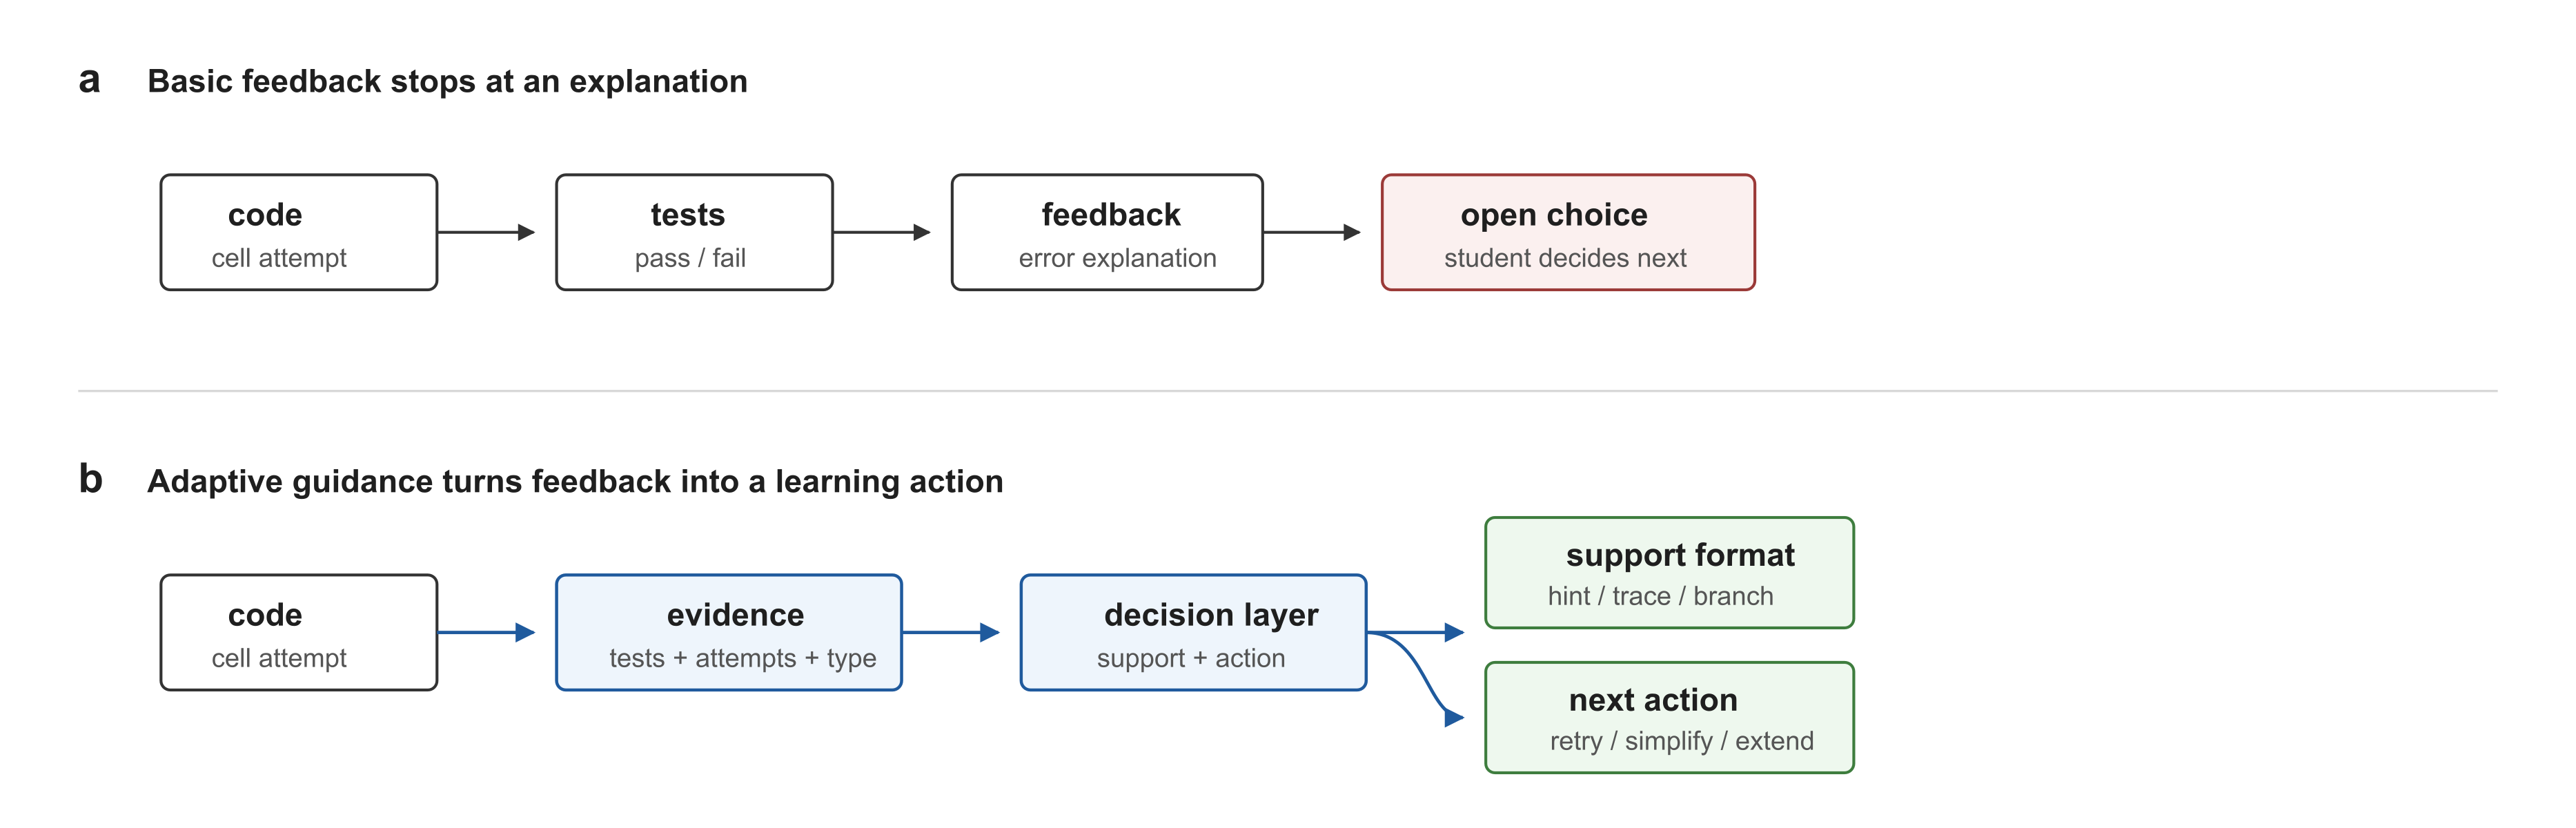
\includegraphics[width=\textwidth]{figure1_basic_to_adaptive.png}
    \caption{\label{fig:basic-to-adaptive}Basic feedback can explain an error; adaptive guidance also recommends support and a next learning action.}
\end{figure}

\section{Existing Work and Gap}

Automated feedback for programming exercises is a well-established area. Reviews of the field show that systems can provide test results, hints, explanations, and correction advice~\cite{Keuning2018,Messer2023}. This gives a useful foundation, but much of the feedback still focuses on the current submission rather than the student's next step.

Next-step hints are closer to my aim, because they try to move the learner forward without simply giving away the answer~\cite{Roest2023,Birillo2024}. My project takes a slightly broader view: the system should decide not only what hint to give, but also what form of support is most useful and whether the next task should be easier, similar, or harder.

Adaptive learning and knowledge tracing are also relevant, although I do not plan to build a full learner model at the start. Corbett and Anderson's knowledge tracing work is useful here because it frames learning as something that can be updated from observed attempts~\cite{Corbett1994}. A lightweight version is enough for the prototype: repeated attempts, repeated mistake types, and recent success can already give useful signals. The project is also shaped by the notebook setting. Jupyter notebooks are widely used for computational work and teaching~\cite{Beg2021}, so I do not want a separate learner dashboard; the support should appear close to the code, where the student is already working.

Cellmate is the practical starting point. Its README describes a VS Code Jupyter Notebook extension that runs hidden tests and generates feedback inside the notebook~\cite{Cellmate2026}. I see it as the feedback layer. My contribution is the decision layer after feedback.

\section{Proposed Method}

The method has two decisions. First, the system chooses a support format. Second, it recommends the student's next learning action. Keeping these separate is important: a student may choose how much help they want, but the system should still decide whether the next exercise should be simpler or harder based on the evidence.

\begin{figure}[htbp]
    \centering
    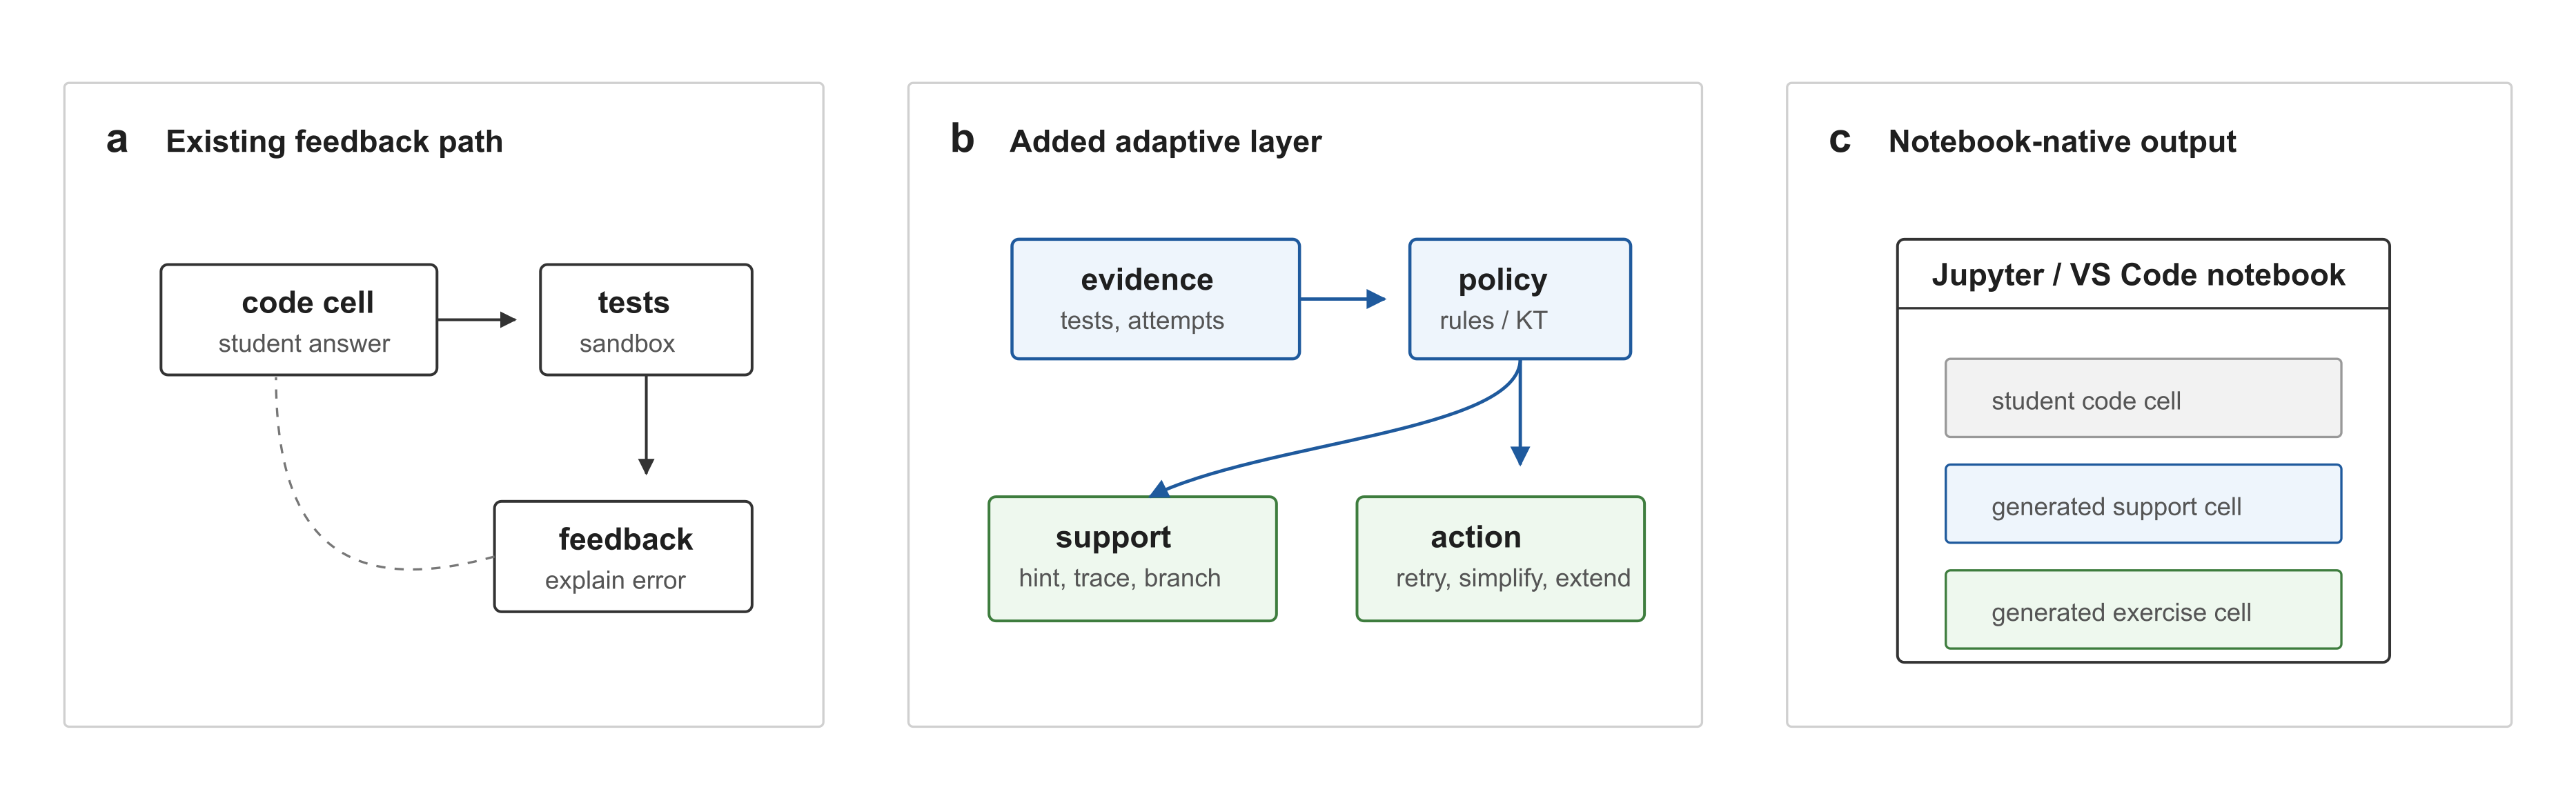
\includegraphics[width=\textwidth]{figure2_system_architecture.png}
    \caption{\label{fig:architecture}The adaptive layer is added after Cellmate-style feedback has been generated.}
\end{figure}

The first version will be rule-based. This is a deliberate choice rather than a shortcut. The rules are inspectable, easy to discuss, and do not depend on expensive external services. Evidence will include hidden test failures, expected versus actual output, attempt count, mistake type, and whether the student succeeds after support. In the prototype, mistake classification will first use task-specific patterns from hidden tests and expected-versus-actual outputs. For example, if a summation task returns the final item rather than the total, the system classifies this as an accumulator update error.

The support mapping below is the starting taxonomy.

\begin{table}[htbp]
    \centering
    \caption{\label{tab:support-mapping}Initial mapping from mistake types to support formats and next actions.}
    \begin{tabular}{lll}
        \toprule
        Mistake type & Support format & Next action \\
        \midrule
        Accumulator update error & State update table & Easier accumulator exercise \\
        Conditional filtering error & Include/exclude comparison & Retry with condition hint \\
        Boundary condition error & Boundary case comparison & Retry with boundary tests \\
        Function return error & Input-output contract & Fix return behaviour \\
        Repeated mistake & Concept reminder & Simpler sub-task \\
        Fast success & Short confirmation & Harder extension \\
        \bottomrule
    \end{tabular}
\end{table}

For example, if the student repeatedly writes \texttt{total = value} in an accumulator task, the system should not immediately send them to a harder task. It should first offer a smaller exercise focused only on updating the running total. If the student passes the hidden tests quickly, the system can generate an extension task instead.

\section{Prototype}

I have built a clickable notebook prototype to make the idea concrete. It is not a full Cellmate extension yet. It is a design prototype that simulates test results, mistake classification, support selection, and follow-up exercise generation inside a notebook-like interface.

\begin{figure}[htbp]
    \centering
    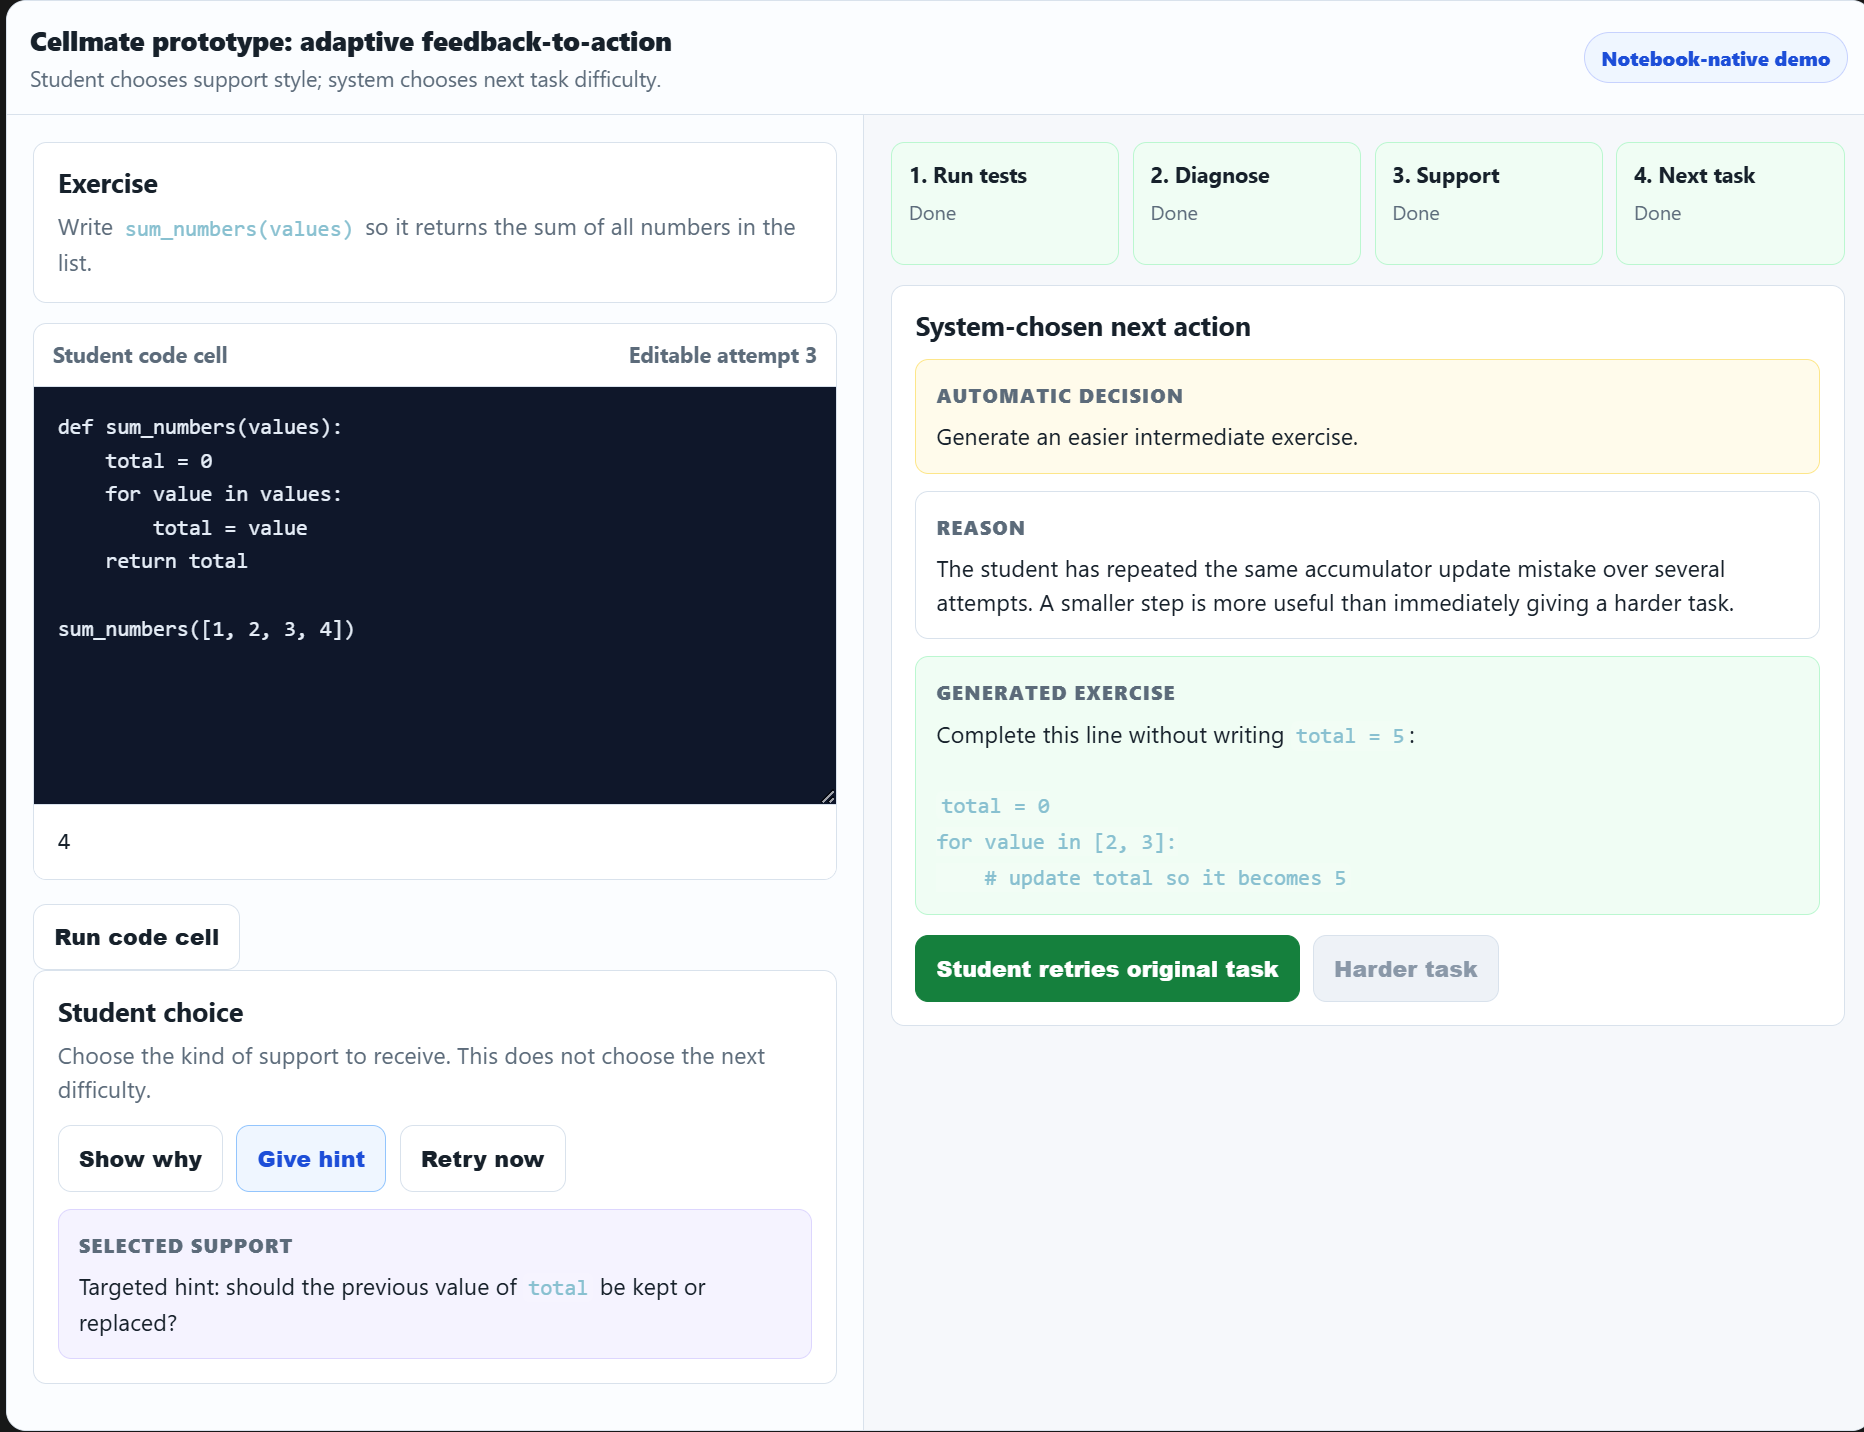
\includegraphics[width=\textwidth]{figure3_prototype_screenshot.png}
    \caption{\label{fig:prototype}Prototype state after a failed accumulator attempt. The system recommends an easier intermediate exercise and disables the harder task.}
\end{figure}

The first example asks the student to write a function that sums a list. The wrong attempt uses \texttt{total = value}, so the function returns the final item rather than the sum. The system classifies this as an accumulator update error. The student can choose a support style such as ``show why'' or ``give hint'', but the task difficulty is decided by the system. Because the same mistake has been repeated, the harder task is disabled and an easier intermediate exercise is generated.

After a successful retry, the prototype generates a harder exercise: summing only positive numbers. This introduces a different mistake type, conditional filtering. If the student adds every value instead of only positive values, the system should not keep showing the same accumulator trace. It should switch to support that explains which values should be included.

\section{Evaluation Plan}

I will compare my version with a simpler version that only gives a correctness result and a short explanation. The purpose is not to prove a large learning effect from a small study, but to check whether the extra guidance helps students decide what to try next.

\begin{figure}[htbp]
    \centering
    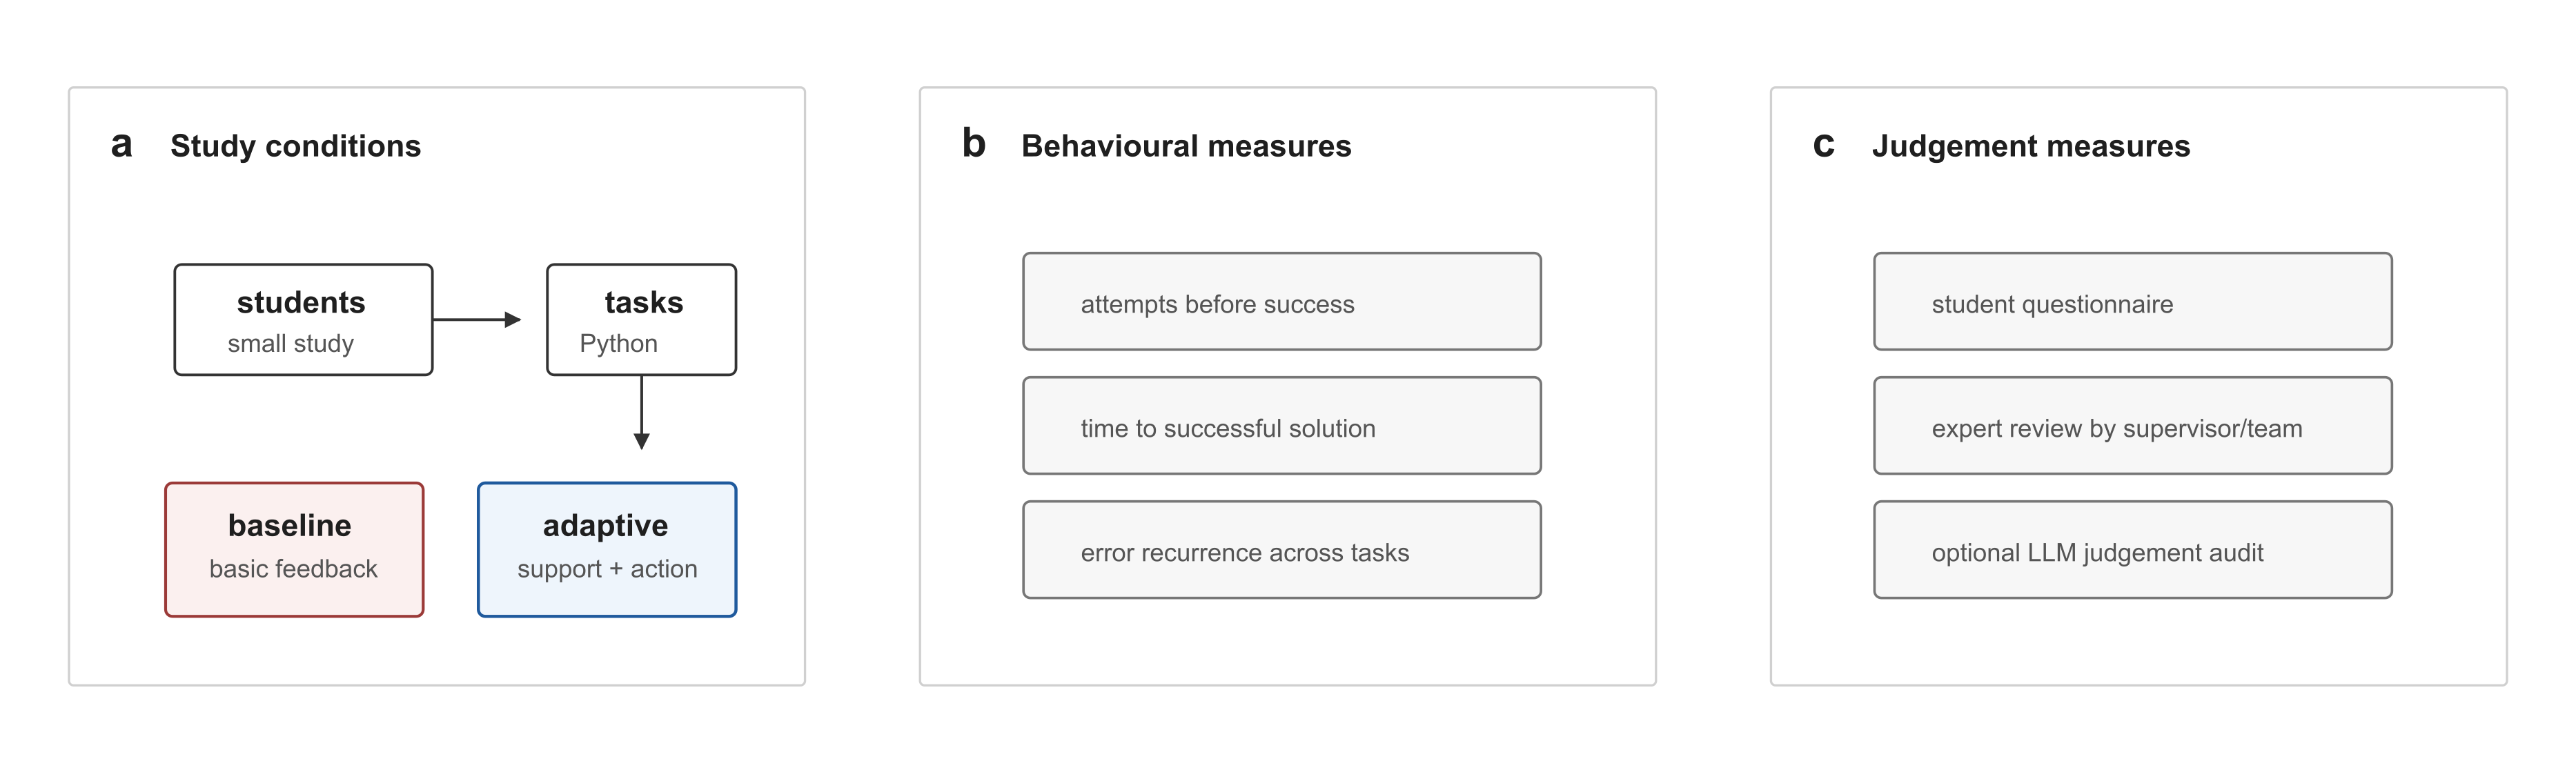
\includegraphics[width=\textwidth]{figure4_evaluation_design.png}
    \caption{\label{fig:evaluation}Planned comparison between ordinary feedback and the version with adaptive guidance.}
\end{figure}

I plan to recruit around 5--8 participants for a small formative within-subject study. Each participant would try comparable tasks in both conditions, with the order counterbalanced where possible to reduce ordering effects. The tasks will focus on accumulators, conditional filtering, and boundary conditions. If participant recruitment is limited, I will use expert review and scripted example cases as a fallback evaluation.

The main measures will be attempts before success, time to success, final success rate, support usage, and whether the same mistake appears again in a later task. I will also use a short questionnaire about clarity, actionability, appropriateness, confidence, cognitive load, and preference. An expert review by the supervisor or project team will judge whether the recommendations are pedagogically sensible and feasible to integrate with Cellmate. If real students are involved, I will collect only minimal anonymous interaction data and follow the required consent and ethics approval process before running the study.

I may also use an LLM as an audit tool. It could rate whether a support format is relevant and whether the next task is too easy or too hard. I would treat this only as supporting evidence, not as a replacement for student behaviour or expert judgement.

\section{Future Plan and Risks}

Month 1 will refine the mistake taxonomy, support matrix, and rule-based decision policy. Month 2 will improve the notebook prototype and make the simulated workflow closer to Cellmate. Month 3 will run the small evaluation or expert review, analyse the results, and write up limitations and future integration.

The main risk is trying to cover too many Python topics. I will manage this by focusing on loops, accumulators, conditionals, and function outputs. Another risk is that real student testing may be limited. If that happens, I will rely more on expert review and carefully designed example cases, while making clear that the evidence is early-stage rather than definitive.

\section{Conclusion}

This project treats feedback as the start of a learning decision, not the end of the interaction. The aim is to help beginner Python learners move from ``my answer is wrong'' to ``this is the next useful thing to try.'' A notebook-native adaptive layer could make tools such as Cellmate more useful after an error while remaining lightweight, transparent, and accessible.

\bibliographystyle{unsrt}
\bibliography{references}

\end{document}
